\documentclass[11.5pt]{sig-alternate} % sets document style to sig-alternate
% packages
% typesetting
%\usepackage{dirtytalk} % typset quotations easier (\say{stuff})
\usepackage{hanging} % hanging paragraphs
\usepackage[defaultlines=3,all]{nowidow} % avoid widows
\usepackage[pdfpagelabels=false]{hyperref} % produce hypertext links, includes backref and nameref
\usepackage{xurl} % defines url linebreaks, loads url package
\usepackage{microtype}
\usepackage{textgreek}
%\usepackage{textcomp}
%\newcommand{\texttildemid}{\raisebox{0.4ex}{\texttildelow}}
% layout
\usepackage{enumitem} % control layout of itemize, enumerate, description
\usepackage{fancyhdr} % control page headers and footers
\usepackage{float} % improved interface for floating objects
%\usepackage{multicol} % intermix single and multiple column pages
% language
\usepackage[utf8]{inputenc} % accept different input encodings
\usepackage[english]{babel} % multilanguage support
% misc
\usepackage{graphicx} % builds upon graphics package, \includegraphics
%\usepackage{lastpage} % reference number of pages
%\usepackage{comment} % exclude portions of text (?)
\usepackage{xcolor} % color extensions
\usepackage[backend=biber, style=apa]{biblatex} % sophisticated bibliographies % necessary for HTML to display author info and date on abstract page
\usepackage{csquotes} % advanced quotations, makes biblatex happy
\usepackage{authblk} % support for footnote style author/affiliation
% tables and figures
\usepackage{tabularray}
%\usepackage{array} % extend array and tabular environments
\usepackage{caption} % customize captions in figures and tables (rotating captions, sideways captions, etc)
%\usepackage{cuted} % allow mixing of \onecolumn and \twocolumn on same page
\usepackage{multirow} % create tabular cells spanning multiple rows
%\usepackage{subfigure} % deprecated, support for manipulation of small figures
%\usepackage{tabularx} % extension of tabular with column designator "x", creates paragraph-like column whose width automatically expands
%\usepackage{wrapfig} % allows figures or tables to have text wrapped around them
%\usepackage{booktabs} % better rules
% dummy text
%\usepackage{blindtext} % blind text dummy text
%\usepackage{kantlipsum} % Kant style dummy text
\usepackage{lipsum} %lorem ipsum dummy text
% other helpful packages may be booktabs, longtable, longtabu, microtype

\pagestyle{fancy} % sets pagestyle to fancy for fancy headers and footers

% header and footer
% modern way to set header image
\renewcommand{\headrulewidth}{0pt} % defines thickness of line under header
\renewcommand{\footrulewidth}{0pt} % defines thickness of line above header
\setlength\headheight{80.0pt} % sets height between top margin and header image, effectively moves page contents down
\addtolength{\textheight}{-80.0pt} % seems to affect the lower height. maybe only works properly if footer numbers enabled?
\fancyhf{}
\fancyhead[CE, CO]{
\includegraphics[width=\textwidth]{headerImage.png}}
% footer
%\fancyfoot[LE,LO]{Article Title Here \\ DOI: }% left footer article title and doi
%\fancyfoot[CE,CO]{{}} % center footer empty
%\fancyfoot[RE,RO]{\thepage} % right footer page numbers
%\pagenumbering{arabic} % arabic (1, 2, 3) numbering in footer

\hypersetup{colorlinks=true,urlcolor=blue} % sets link color to blue
\urlstyle{same} % sets url typeface to same as rest of text

% set caption and figure to italics, label bold, left align captions, does not transfer to HTML
\captionsetup{labelfont=bf, font={large, it}, justification=raggedright, singlelinecheck=false}
\renewcommand\theContinuedFloat{\alph{ContinuedFloat}}

%this next bit is confusing, but essentially changes the width of the abstract. Seems to have been copied from this https://tex.stackexchange.com/questions/151583/how-to-adjust-the-width-of-abstract
\let\oldabstract\abstract
\let\oldendabstract\endabstract
\makeatletter %changes @ catcode to enable modification (in parsep)
\renewenvironment{abstract} %alters the abstract environment
{\renewenvironment{quotation}%
               {\list{}{\addtolength{\leftmargin}{1em} % change this value to add or remove length to the the default ?
                        \listparindent 1.5em%
                        \itemindent    \listparindent%
                        \rightmargin   \leftmargin%
                        \parsep        \z@ \@plus\p@}%
                \item\relax}%
               {\endlist}%
\oldabstract}
{\oldendabstract}
\makeatother %changes @ catcode to disable modification

% checks
% italics
% links
% dashes
% tildes
\begin{document}

\title{The Next Generation Laboratory Interface for Students with Blindness or Low Vision in the Science Laboratory}

\author[1]{\large \color{blue}Cary A. Supalo}

\affil[1]{Illinois State University}

\toappear{}
%% ABSTRACT
\maketitle
\begin{@twocolumnfalse} 
\begin{abstract}
\item 
\textit{Entry into science education for students with blindness or low vision can present economic and technological barriers to access. This manuscript discusses funding hands-on student experiences in middle school, high school, and post-secondary education. Further, the use of access technologies recently developed for science education is also presented. Partnerships between access technology companies that are committed to working together make access more possible than ever before. The shift from the Director Assisted Approach to independent data collection in a hands-on way to promote interest in Science, Technology, Engineering, and Mathematics (STEM) careers is discussed.}
\\ \\

\end{abstract}
\end{@twocolumnfalse}

%% AUTHOR INFORMATION

\textbf{*Corresponding Author, Cary A. Supalo}\\
\href{mailto: casupal@ilstu.edu }{(casupal@ilstu.edu)} \\
\textit{Submitted  Dec 18 2013}\\
\textit{Accepted Dec 18 2013} \\
\textit{Published online Dec 18 2013} \\
\textit{DOI:10.14448/jsesd.05.0004} \\
\pagebreak
\clearpage
\begin{large}

Students with blindness or low vision (BLV) have traditionally been marginalized in their direct hands-on involvement in the science laboratory. It had previously been perceived that due to the lack of vision, safety and other related concerns, their full participation and integration into the hands-on active aspects of a laboratory experience were thought to be unwise and not safe (Swanson \& Steele, 1981). A common solution to this challenge was to provide a person designated as a laboratory assistant who would serve as the student with BLV’s hands and eyes in the laboratory (Miner, Nieman, Swanson, \& Woods, 2001). This has been referred to as the, “Director Assisted Approach.” This approach requires the student with BLV to verbally instruct the assistant as to the specific aspects of the laboratory procedure. The assistant then describes the results of those specific actions. The student with BLV is responsible for data recording, and if print or hand written observations are also required, then it is up to the student with BLV to instruct the assistant as to what to record in the laboratory notebook. The role of the assistant can be either fulfilled by a classmate or other volunteer. A major disadvantage to the classmate’s serving in the role as an assistant is that it takes away from the opportunity this student has to contribute intellectually to the laboratory experience. Further, a disadvantage to working with a volunteer is that this individual may not be as committed to this opportunity because he/she views it more as an act of charity than a job. Therefore, a paid position is most ideal. This can commonly be done at the post-secondary level by an office for disability concerns or equivalent. Sometimes specific departments can also be asked to provide some funds for this type of accommodation in a research laboratory experience. Funding may also be sought from the student with BLV’s vocational rehabilitation counselor. Vocational rehabilitation agencies are funded by the United States’ department of Education under the Rehabilitation Services Administration (RSA) (Willoughby \& Duffy, 1989). The premise for these funds is viewed as an investment in the student with a disability to become employable and thus would achieve a lifelong career in a field of their choice thus allowing them to contribute to the workforce and pay taxes. However, funding resources vary from institution to institution. Therefore, the creativity of the student with BLV and the faculty he/she is working with is important to a successful hands-on learning experience.

In the early 1980’s, research led by William J. Skawinski at the New Jersey Institute of Technology developed a project known as, “Macrolab” (Cochin \& Herman, 1981). This effort developed a series of talking laboratory probes such as pH, balance, and temperature sensors to be used in the science laboratory. Although these tools were innovative for the time, they were never mass produced due to high cost to replicate. Later, Lunney et al (1996) successfully interfaced a portable electronic note taker referred to as Braille ‘N Speak distributed by Blazie Engineering in the early 1990s with common electronic laboratory equipment equipped with RS-232 ports \& ASCII output capability. This interface, although far more cost effective, was difficult to replicate due to customization needed in pin configurations on connector cables between laboratory equipment and the Braille ‘N Speak device. Later, Supalo et al obtained a National Science Foundation Research in Disabilities Education (RDE) grant to found the Independent Laboratory Access for the Blind (ILAB) project (Supalo, 2010; Supalo, 2007; Supalo, Mallouk, Amorosi, Lanouette, Wohlers, \& McEnnis, 2009; Supalo, Mallouk, Amorosi, Rankel, Wohlers, Roth, \& Greenberg, 2007).This initiative sought to develop a suite of talking and audible laboratory tools to be first used in high school chemistry and later other science courses. The ILAB team partnered with Vernier Software \& Technology to incorporate text-to-speech accessibility support for one of the largest laboratory sensor computer interfaces to be used in secondary science laboratory classrooms across the United States. The Vernier hardware interfaced with a scientific data collection software package known as Logger Pro. This software driven interface empowers students to obtain highly quantifiable data sets. Further, it enables all students to perform higher functional statistical analysis on multiple data sets. Having quantifiable data enhances student laboratory learning experiences to more fully explain the science concepts being taught. 

The ILAB team contracted with a software engineer to produce an interface between the Job Access with Speech (JAWS) text-to-speech screen reader distributed by Freedom Scientific and the Logger Pro scientific data analysis program distributed by Vernier Software \& Technology. This JAWS/Logger Pro interface was later emulated to work with the Window-Eyes text-to-speech screen reader distributed by G.W. Micro. The Window Eyes compatibility with Logger Pro was due to a partnership between G.W. Micro and Independence Science, a science access technology company founded by Supalo. G.W. Micro has made a firm commitment to ensure science access for students with BLV in the science laboratory.

The Jaws/Logger Pro interface was field tested over the six year period in fifteen schools across the United States (Supalo, Humphrey, Mallouk, Wohlers, \& Carlsen, 2013). Feedback was collected from ILAB research participants and provided to software engineers to make revisions for the next academic year. Upon the conclusion of the ILAB project, no more financial support was available to maintain the JAWS/Logger Pro script files necessary. Therefore, a partnership with G.W. Micro to support and maintain a similar interface was established.

\section*{VERNIER SOFTWARE \& TECHNOLOGY LAB\-QUEST}

In 2007, Vernier Software \& Technology launched a new product known as the LabQuest. This handheld computer (figure 1) serves as one of the first portable scientific data collection devices. This handheld computer successfully interfaces with most of the Vernier product line of laboratory sensors. Students no longer need a laptop computer to collect and analyze scientific data. The LabQuest is a powerful tool in an informal science learning setting and allows students to take quantifiable data in the field. This new innovative piece of hardware is equipped with a touch screen, microphone and headphone jacks, onboard rechargeable battery, and USB, USB mini, and SD card slots for expanded data storage. Additionally, there are four analog and two digital probe ports for Vernier sensors. There is also an internal microphone and speaker. Supalo, when he first saw the LabQuest, had the idea of wanting to develop a text-to-speech screen reader for the LabQuest. This would create the first accessible portable scientific data collection device for students with BLV. In 2009, Supalo’s firm Independence Science applied for and successfully obtained a National Science Foundation Small Business Innovation Research (SBIR) grant to develop an alpha version of a text-to-speech screen reader for the LabQuest (Isaacson, Supalo, \& Lloyd, 2013; Supalo, Isaacson \& Lombardi, 2013). An educational research study was conducted at a residential school for the blind to field test the alpha version of this software application. A large majority of students with BLV from the sample of 27 participants indicated positive feedback towards the use of text-to-speech as compared to non-talking LabQuest technologies.

\begin{figure}[h]
    \centering
    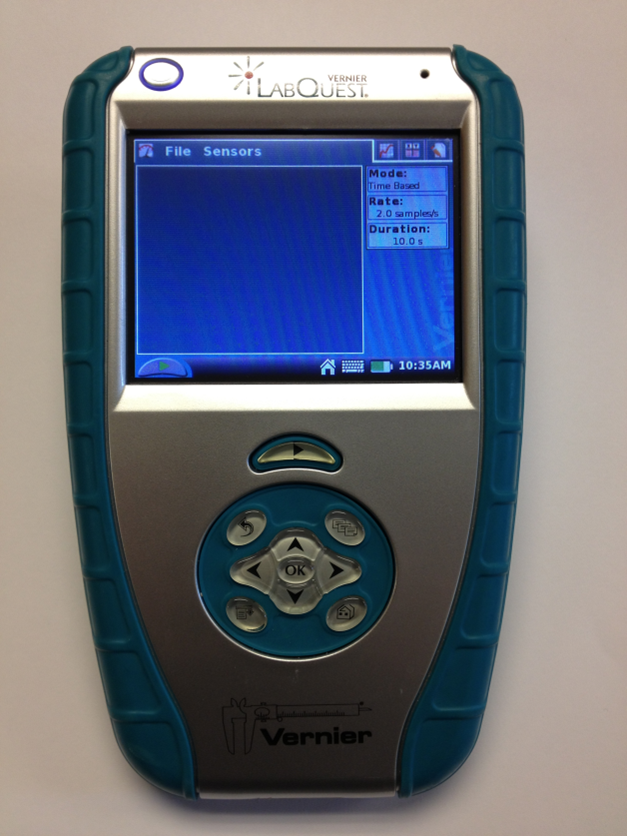
\includegraphics[width=1\linewidth]{images/fig1.png}
    \caption{Vernier Software \& Technology LabQuest}
\end{figure}
 
These findings led Independence Science to apply for and successfully obtain an NSF-SBIR phase II award with the intent of development of further functionality and led to commercialization of the Talking LabQuest device. In December 2011, Independence Science made the Talking LabQuest publicly available. This device was sold as a product under development. All early adopters would receive free software upgrades through the end of 2013 at which time the NSF funding would conclude. Therefore, this would ensure all customers would have full benefit of the R\&D efforts by Independence Science no matter when they purchased the devices.

\section*{SCI-VOICE TALKING LABQUEST}

The original LabQuest device has a series of buttons located on the top face of the device. These buttons are shown in figure 2. There are four navigation buttons shaped like arrows along with a center button that serves as the OK button. The meaning of the arrow buttons is implied to indicate up, down, left, and right screen navigation. The four corner buttons serve as a main menu button that contains a picture of a house on it. The lower left button is the file menu button. The top right button serves as the page forward button as the LabQuest contains four different pages titled, “sensor, graph, data table page, and notes page.” The top left button serves as the back button between screens. These buttons allow a student with BLV to have full navigation capabilities on all dialog boxes and menus on the LabQuest device. Further, an accessibility menu was added under the preferences submenu in the control panel to give a student with BLV control over the text-to-speech. These controls include, gender, speech rate, pitch, and tone. Further, localization efforts are under way to enable the LabQuest device to speak multiple languages. Other text-to-speech engines are being investigated for internationalization opportunities.

\begin{figure}[h]
    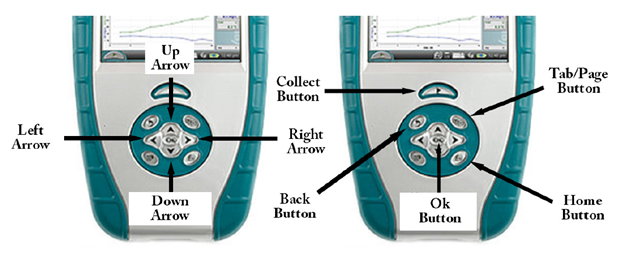
\includegraphics[width=1\linewidth]{images/fig2.png}
    \caption{Figure 2. – Close View of Sci-Voice Talking LabQuest Navigation Buttons.*}
    \begin{large}\textit{ *Image borrowed from Talking LabQuest Quick Start Guide by Independence Science.}\end{large}
\end{figure}

The Sci-Voice talking LabQuest also has an accessible periodic table of the elements application that can be accessed from the main menu. This talking periodic table application allows a student with BLV to navigate by means of arrow keys around the periodic table thus providing a physical geographical layout of how the elements are related from one to another between the columns and rows. Further, the OK button can be used to pull up a list box of approximately 20 facts on every element on the periodic table. These facts can range from atomic mass, atomic number, first ionization energy, electron configuration, visual appearance, discovery date, and who discovered it. There is also a talking scientific calculator application found on the Sci-Voice Talking LabQuest’s control panel. This feature can be utilized by students with BLV. 

It is for these reasons that the Sci-Voice Talking LabQuest is one of the most useful science laboratory devices for students with BLV. Since the Sci-Voice Talking LabQuest interfaces with approximately 70 Vernier sensors from all sciences, this device is opening doors of opportunity for students with BLV and other students with print disabilities to have access to quantifiable scientific data.

The Sci-Voice Talking LabQuest promotes hands-on science learning experiences for students with BLV to consider career paths in Science, Technology, Engineering, and Mathematics (STEM). Through hands-on science learning experiences students with BLV are learning science by doing. It is this learning by doing approach further reinforced by Piaget (1970) that shows learning through participation leads to independence in the science laboratory. It is this perceived independence in the science laboratory that encourages more students with BLV to consider career paths in STEM.

\section*{ACKNOWLEDGEMENTS}

The author would like to acknowledge the National Science Foundation RDE program for providing funding under award numbers HRD-RDE 0726417 and HRD-RDE 0435656 for support of the ILAB project

Further, the author would like to acknowledge the NSF for financial support for SBIR award numbers 0945481 and 1127412 for support of the Sci-Voice Talking LabQuest 

Credit goes to Vernier Software \& Technology for without its significant contributions to the ILAB and Sci-Voice Talking LabQuest projects, none of this would be possible. 

Additional Credit goes to G.W. Micro for their ongoing support of the Window-Eyes Logger Pro interface

\section*{BIOGRAPHICAL STATEMENTS}

Cary A. Supalo \href{mailto:casupal@ilstu.edu}{(casupal@ilstu.edu)}, completed his Ph.D. in chemistry, with an emphasis in chemical education, in fall 2010 at The Pennsylvania State University. He cofounded ILAB in 2004 and managed the project for the six years of its active existence. For his dissertation, he field tested the ILAB tools in 12 mainstream high schools across the U.S. and is currently completing analyses of the data. In 2009 he founded and is president of Independence Science LLC, a business offering consulting services and assistive hardware/software to school districts, state rehabilitation agencies, colleges and universities, and students and parents. In helping students with blindness or low vision to have hands-on science learning experiences, Independence Science is continuing the work begun during the ILAB project. The Next Generation Laboratory Interface for Students with Blindness or Low Vision in the Science Laboratory

\end{large}
\clearpage
\section*{REFERENCES}\par 

\leftskip 0.25in
\parindent -0.25in 
Cochin, I.; Herman, H. (1981). The Macrolab: A Center for the Handicapped at NJIT. NSF award number SPI-7908704. New Jersey Institute of Technology and the Foundation at NJIT, Newark, NJ.

Isaacson, M.; Supalo, C.; Lloyd, L. (n.d.). (2013). Hands-on science experiences for students with visual impairments and STEM motivation. \textit{Journal of Visual Impairment and Blindness}, in review.

Lunney, D.; Gemperline, M.; Sonnesso, A.; Wohlers, D. (1996). Research Note: The Braille ’N Speak As a Laboratory Tool for Blind Students. \textit{Information Technology and Disabilities, 3} (1).

Miner, D.; Nieman, R.; Swanson, A.; Woods, M. (2001). Teaching Chemistry to Students with Disabililties: A Manual for High Schools, Colleges, and Graduate Programs. Washington, D.C: American Chemical Society

Piaget, J. (1970). Science of Education and the Psychology of the Child. New York: Orion Press.

Supalo, C. (2007). Independent Laboratory Access for the Blind. \textit{Braille Monitor, 50} (5)

Supalo, C..; Mallouk, T..; Amorosi, C.; Rankel, L.; Wohlers, D.; Roth, A.; Greenberg, A. (2007). Talking Tools to Assist Students Who Are Blind in Laboratory Courses. \textit{J. of Sci. Educ. for Students with Disabilities, 12} (1), 27-32.

Supalo, C..; Mallouk, T.; Amorosi, C.; Lanouette, J.; Wohlers, D.; McEnnis, K. (2009). Using Adaptive Tools and Techniques to Teach a Class of Students Who Are Blind or Low-Vision. \textit{J. Chem. Educ., 86} (5), 587-591.

Supalo, C. (2010). Teaching Chemistry and Other Sciences to Blind and Low-Vision Students Through Hands-On Learning Experiences in High School Science Laboratories. Ph.D. Dissertation, Pennsylvania State University.

Supalo, C; Isaacson, M.; Lombardi, M. (2013). , Mick D. Isaacson, Michael V. Lombardi  Making Hands-On Science Learning for Students Who Are Blind or Have Low Vision. \textit{J. Chem. Educ.}, in review.

Supalo, C.; Humphrey, J.; Mallouk, E.; Wohlers, D.; Carlsen, S. (2013). Examining the Use of Adaptive Technologies in Increasing the Hands-On Participation of Students with Blindness or Low Vision in Secondary-School Chemistry and Physics, \textit{J. Chem. Educ.}, in review.

Swanson, A; Steere, N. (1981). Safety considerations for physically handicapped individuals in the chemistry laboratory.  \textit{J. Chem. Educ., 58} (3), 234

Willoughby, D.; Duffy, S. (1989). Handbook for Itinerant and Resource Teachers of Blind and Visually Impaired Students. Baltimore: National Federation of the Blind, 327-330.



\end{document}
